\documentclass[a4paper]{article}
\usepackage[utf8]{inputenc}
\usepackage{geometry}
\usepackage{graphicx}
\usepackage{subfigure}
\geometry{a4paper,scale=0.85}

\title{Fast Solvers for Large Systems of Equations}
\author{Shuai Lu 170742}
\date{Homework 5}

\begin{document}
\maketitle
\noindent \textbf{Exercise 5.1*} Perform computations with the problem, grid and solvers from Exercise 4.2(a) with $d=0.0001$ in the stripe on the refinement level 6 using the script $diff\_with\_stripe\_sm.lua$. In this script, the linear iteration preconditioned by the geometric multigrid method (V-cycle) with the ILU smoother is used.\\

\noindent (a) [2 points] Test different numbers of the pre- and postsmoothing steps by choosing $n=1, \ldots, 6$. (Use command line option "-numSmooth $n$ ".) For every of these values, report the number of the iterations, the final convergence rate and the time spent by the solver. (The solver time is printed by the script.) For which $n$ the time is minimal? And for which $n$, the number of the iterations is minimal? Explain why these are not the same settings?\\

\noindent Solution:\\
\noindent The result is shown in Fig.1. The time is minimal when $n=2$. The number of the iterations is minimal when $n=6$. Although more smoothing steps will reduce the iteration, the cost of smoothing will increase as well. So there is a trade off between numbers of iteration and smoothing steps to minimize the running time. \\
\begin{figure}[htbp]
	\centering
	\begin{minipage}[t]{0.7\textwidth}
		\centering		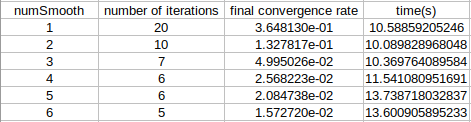
\includegraphics[width=10cm]{5.1a.png}
		\caption{The test result of different numSmooths}
	\end{minipage}
\end{figure}

\noindent (b) [2 points] Try $n=0$ What happens? Explain this phenomenon.\\

\noindent Solution:\\
\noindent It can not converge. There is no smoothing step to reduce the high error frequencies.\\

\noindent \textbf{Exercise 5.2} Perform the computations from Exercise $5.1$ with two pre- and postsmoothing steps (default value in the script) with the other smoothers and the other grids:\\

\noindent (a) [2 points] Use the -smoother option with ilu (for the ILU decomposition), jac (for the Jacobi smoother with the damping parameter $\theta=0.66$ ) and gs (for the Gauss-Seidel smoother). Repeat the same computations on the grid stripe1.ugx (use command line option -grid stripe1.ugx). Note that this grid is worse. (Why?) For every of these tests, report the number of the iterations, the final convergence rate and the time spent by the solver. Compare the results for the different smoothers and grids.\\

\noindent Solution:\\

\noindent The result is shown in Fig.2. The number of iteration is minimal when using ILU smoother but its running time is the maximal under the same grid. The number of iteration is maximal when using Jacobi smoother but its running time is the minimal under the same grid. Fixing the smoother, the performance of using the grid stripe.ugx is always better  than that of using the grid stripe1.ugx. The level0 grids in stripe.ugx and stripe1.ugx are shown in Fig.3 and 4. It is obvious that the angle of triangle in stripe1.ugx is sharper than that in stripe.ugx. And this bad condition can not be improved by refining the mesh normally.\\

\begin{figure}[htbp]
	\centering
	\begin{minipage}[t]{0.7\textwidth}
		\centering		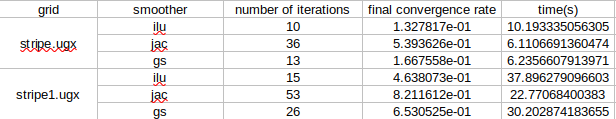
\includegraphics[width=10cm]{5.2a.png}
		\caption{The test result of different smoothers and grids(linear iteration)}
	\end{minipage}
\end{figure}

\begin{figure}[htbp]
	\centering
	\begin{minipage}[t]{0.7\textwidth}
		\centering		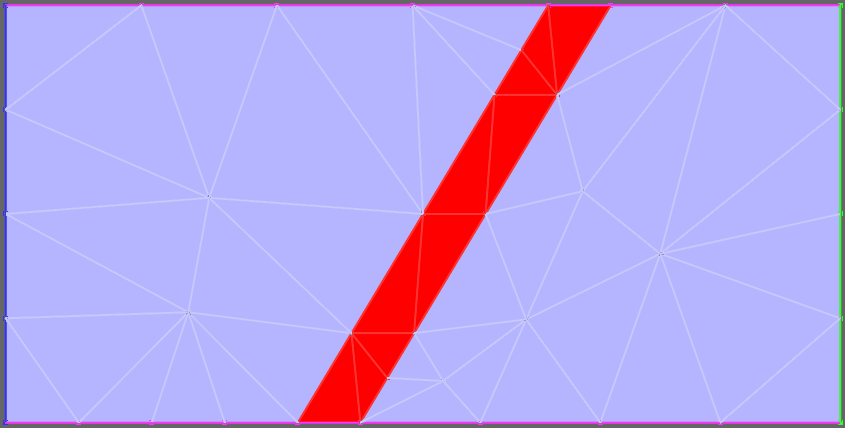
\includegraphics[width=10cm]{stripe.png}
		\caption{Basic mesh in stripe.ugx}
	\end{minipage}
\end{figure}
\begin{figure}[htbp]
	\centering
	\begin{minipage}[t]{0.7\textwidth}
		\centering		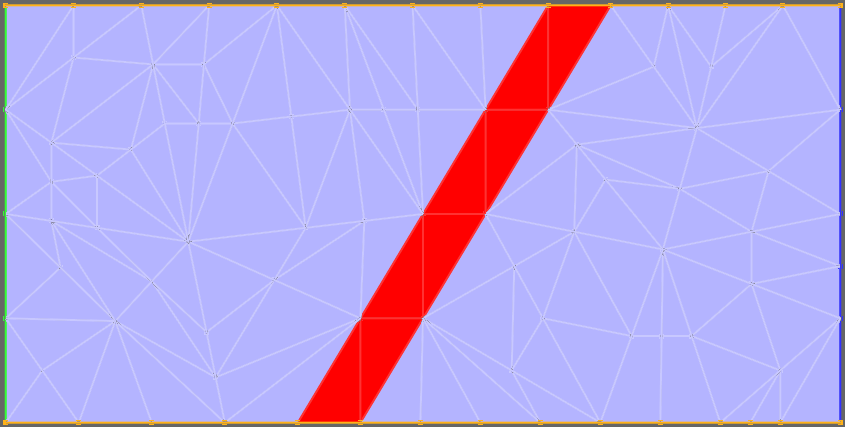
\includegraphics[width=10cm]{stripe1.png}
		\caption{Basic mesh in stripe1.ugx}
	\end{minipage}
\end{figure}

\noindent (b) [1 point] Repeat the computations from Ex. $5.2(a)$ on the two grids with the ILU and the Jacobi smoothers but inside of the GMG preconditioner in the CG iteration (use the -solver cg option). For every of these tests, report the number of the iterations, the average convergence rate and the time spent by the solver. Compare the results for the different smoothers and grids.\\

\noindent Solution:\\
\noindent The result is shown in Fig.5. The conclusion is similar to that in (a). The number of iteration is minimal when using ILU smoother but its running time is the maximal under the same grid. The number of iteration is maximal when using Jacobi smoother but its running time is the minimal under the same grid. Fixing the smoother, the performance of using the grid stripe.ugx is always better  than that of using the grid stripe1.ugx.\\

\begin{figure}[htbp]
	\centering
	\begin{minipage}[t]{0.7\textwidth}
		\centering		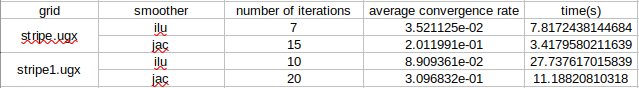
\includegraphics[width=10cm]{5.2b.png}
		\caption{The test result of different smoothers and grids(CG iteration)}
	\end{minipage}
\end{figure}

\noindent \textbf{Exercise 5.3} Simulate the isotropic diffusion on an anisotropic mesh using the script $aniso\_refinement.lua$. In this script, the linear iteration preconditioned by the geometric multigrid method (V-cycle) with the ILU smoothers is applied, too. Before the computations, have a look at the grid in $anisotropic\_grid.ugx$. For every experiment, report the number of iterations, the average convergence rate of the solver and the norm of the last defect.\\

\noindent (a) [1 point] Run the script without any command line options. It computes the solution on the grid level 6 (66049 nodes) with the isotropic refinement strategy. View the created grid hierarchy in $iso\_grid\_hierarchy\_GL6.ugx$. Report the number of the iterations and the final convergence rate.\\

\noindent Solution:\\

\noindent The created grid hierarchy is shown in Fig.6. The number of iteration is 51. The final convergence rate is 7.981626e-01.\\

\begin{figure}[htbp]
	\centering
	\begin{minipage}[t]{0.7\textwidth}
		\centering		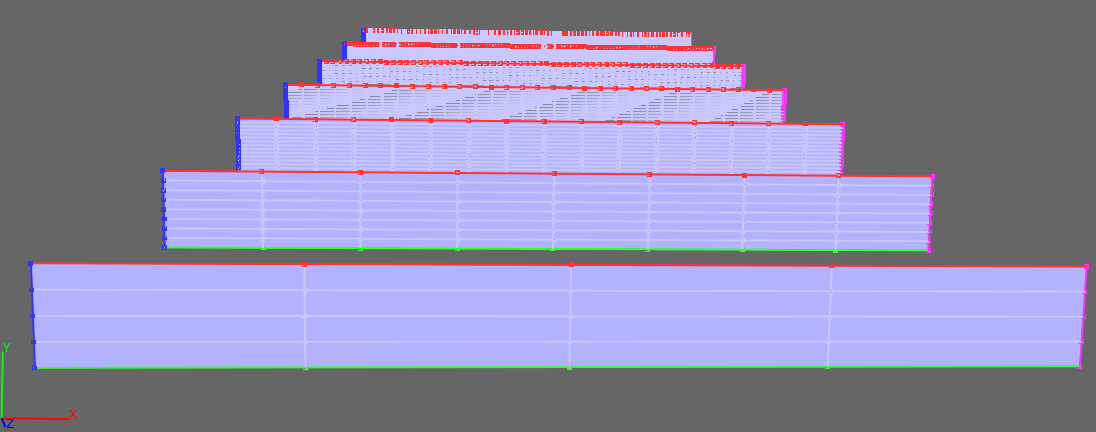
\includegraphics[width=10cm]{grids.png}
		\caption{The grid hierarchy(numRefs=6)}
	\end{minipage}
\end{figure}

\noindent (b) [2 points] Run the script with options "-anisotropic true -numRefs 7". Then it computes the solution on grid level 7 (66177 nodes) with the first 2 refinements being anisotropic. (After these refinements, the aspect ration of the grid elements is reduced.) View the created grid hierarchy in $aniso\_grid\_hierarchy\_GL7.ugx$. Report the number of the iterations and the final convergence rate. Why do we need to increase the number of the grid levels to retain the number of the grid points on the finest grid?\\

\noindent Solution:\\
\noindent The created grid hierarchy is shown in Fig.7. The number of iteration is 5. The final convergence rate is 5.513960e-02. Usually, we compare the computational performance under the same degree of freedom. There are 66049 nodes on isotropic refinement grid level 6, so we need to increase the anisotropic refinement grid level to 7 (66177 nodes).\\

\begin{figure}[htbp]
	\centering
	\begin{minipage}[t]{0.7\textwidth}
		\centering		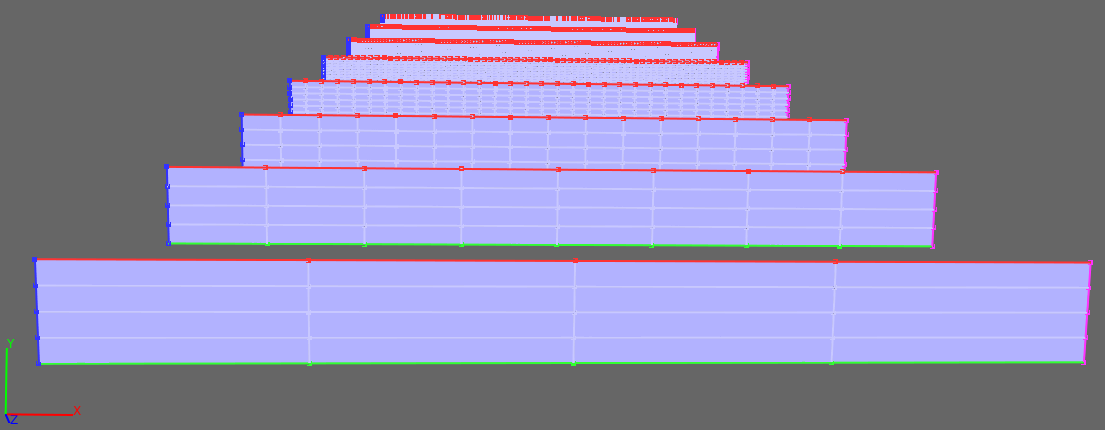
\includegraphics[width=10cm]{grid7.png}
		\caption{The grid hierarchy(numRefs=7)}
	\end{minipage}
\end{figure}

\noindent (c) [1 point] Run the script with "-anisotropic true -numRefs 8 -numAnisoRefs 4". Then it computes the solution on grid level 8 (13225 nodes) with the first 3 refinements being anisotropic. Then the aspect ration of the fine grid elements is close to 1 . View the created grid hierarchy in file $aniso\_grid\_hierarchy\_GL8.ugx$. Report the number of the iterations and the final convergence rate.\\

\noindent Solution:\\
\noindent The created grid hierarchy is shown in Fig.8. The number of iteration is 4. The final convergence rate is 4.179660e-03.\\

\begin{figure}[htbp]
	\centering
	\begin{minipage}[t]{0.7\textwidth}
		\centering		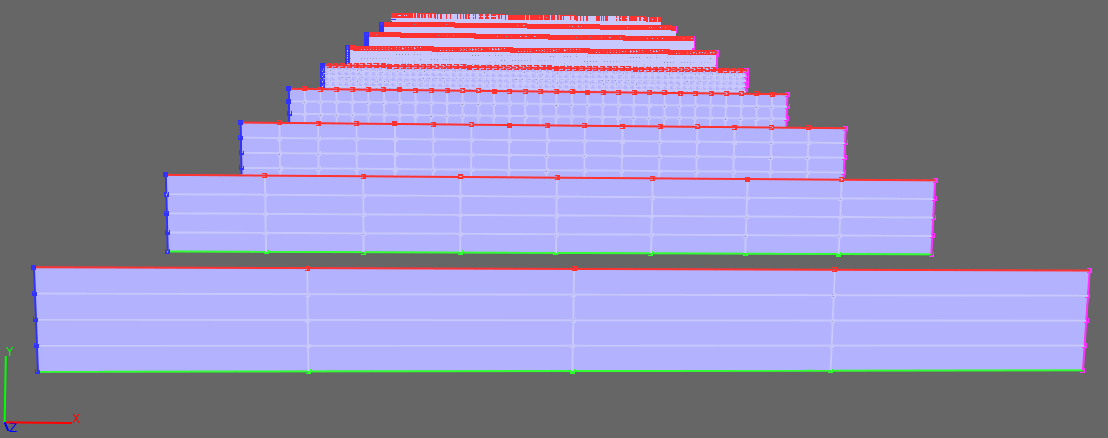
\includegraphics[width=10cm]{grid8.png}
		\caption{The grid hierarchy(numRefs=8)}
	\end{minipage}
\end{figure}

\noindent \textbf{Exercise 5.4*} [4 points] Consider a boundary value problem for an elliptic equation on $\Omega=(0,1)^{2}$. Let this problem be discretized (by FE, FV or FD) on the equidistant cartesian $(N+1) \times(N+1)$-grid $\Omega_{h}$, so that $N=2^{l}$. Estimate (in the $O\left(N^{\alpha}\right)$-form) the amount of computational work for the geometric multigrid $\mathrm{V}(1,1)$-cycle as a preconditioner on this grid. Assume that on a $(M+1) \times(M+1)$-grid, the smoother requires $O\left(M^{2}\right)$ arithmetical operations. Furthermore, the coarse grid solver is applied on the $3 \times 3$-grid of the hierarchy.\\

\noindent Solution:\\
\noindent For the $l$ level, presmoothing requires $O(N^2)$ arithmetical operations. For the $l-1$ level, presmoothing requires $O(\frac{N^2}{4})$ arithmetical operations. The number will decrease by the factor $\frac{1}{4}$ until 2 level, where presmoothing requires $O(\frac{N^2}{4^{l-2}})$ arithmetical operations. The same for restriction, prolongation and postsmoothing. So we need approximate $O(\frac{16}{3}N^2)$ arithmetical operations in total. The amount of computational work is $O(N^2)$\\

\end{document}.